\documentclass[reprint,amsmath,amssymb,aps,superscriptaddress,nofootinbib]{revtex4-2}
\usepackage{graphicx}
\usepackage{booktabs}
\usepackage{array}
\usepackage[T1]{fontenc}
\usepackage[utf8]{inputenc}
\usepackage{hyperref}
\hypersetup{pdftitle={A Readout Is Not an Idle: Phase, Coherence and Concurrence Costs to Untouched Qubits on IBM Processors}}
\newcommand{\us}{\,$\mu$s}
\newcommand{\ket}[1]{$|#1\rangle$}

\begin{document}

\title{A Readout Is Not an Idle: Phase, Coherence and Concurrence Costs to Untouched Qubits on IBM Processors}

\author{K. Indahl}
\email{Indahl@heuremen.com}
\affiliation{Heuremen LLC}

\date{October 30, 2026}

\begin{abstract}
We compare mid-circuit readouts with idles of the same scheduled length in the same job on IBM 156-qubit processors. With 39 of 156 qubits read out, the phase of the 117 untouched qubits is kicked by 1.7 to 2.4$^\circ$ per readout on four processors (analysis defined after the data), and by 1.6 to 2.9$^\circ$ on three in an independent control run whose analysis was fixed before its data were opened, in a layout with every untouched qubit within two couplings of a measured one. The kick is not an advance along each qubit's own precession (qubits that precess the other way are kicked the same way; an extra readout time above 4, 1 and 12\% of the stated length is excluded on fez, kingston and marrakesh, a bound defined after the data), is not larger with the measured qubits in $|1\rangle$, and depends on how many of the 39 are read out, not in proportion (one of 39 read out leaves at most 0.15$^\circ$ on fez and marrakesh and 0.09$^\circ$ on kingston, marrakesh by a copy-gap reading defined after the data; 10 of 39 give 8 to 10\% of the kick pooled per processor (11\% in a fez repeat; upper interval ends 14 to 21\%) against 26\% if proportional; one random subset of each size). It reaches qubits three to four couplings from the measured ones (0.8 to 1.8$^\circ$ with the 39 packed together, 15 qubits in one layout; 0.1 to 0.4$^\circ$ four couplings away in three other layouts, pooled per processor, with per-layout medians differing several-fold), shows no resolved wear-out over 72 readouts against equal idles, and is mostly removed by a symmetric echo (residual resolved on all three, opposite in sign on kingston). These sizes are for the default \texttt{measure} instruction; the shorter \texttt{measure\_2} gives 0.51 to 0.58 of the kick on ibm\_marrakesh, 0.95 to 1.01 on ibm\_kingston (in repeats meeting the known-good rule; no reduction resolved, the length-proportional 0.63 excluded), and cannot tell on ibm\_fez. Equal-idle runs two weeks earlier, with 5 to 25 measured qubits and recomputed after the data, resolve a kick of 0.3 to 3.1$^\circ$ per readout within two couplings in 18 of 25 arms. Readouts also cost untouched qubits coherence (0.004 to 0.021 after 2 to 8 readouts with every measured neighbour verified in $|0\rangle$; resolved on kingston and marrakesh, on fez only at 2 readouts and by a copy-gap reading defined after the data; a neighbour hidden in a level that reads as 0 is excluded on marrakesh only) and untouched Bell pairs concurrence of their X part, which a fixed local rotation can also lower (0.005 to 0.010 after 4 readouts, clean-shot reading, in two runs; kingston by a copy-gap reading defined after the data; selection can bias the loss upward). At equal elapsed time a measured qubit on ibm\_fez keeps 0.48 to 0.52 of its signal after 24 readouts where idling leaves 0.62 to 0.66. Idle decay leaves 62 to 85\% of qubit-copies below their own exponential at 30\us{} (a per-qubit systematic common to the copies is not excluded); at intervals of 30\us{} and longer this removes most of the few-percent excess after spaced X-gate trains (over-correcting by 1 to 2\% on marrakesh), and a model with a fitted rate spread reproduces the measured negative per-gate residual (model 1.3 times the measured size), which on fez and kingston an extra-gate test shows is not a gate cost. On one Rigetti processor a neighbour in $|2\rangle$ shifts a coupled qubit's precession rate by $-54.93\pm1.28$ and $-38.64\pm1.62^\circ$/\textmu s (shot noise only) on two dates between which the pulse amplitude, the number of simultaneous qubits and the calibration all changed.
\end{abstract}

\maketitle

\section{Introduction}

A dispersive readout of a transmon populates a resonator, rings up and down, and dephases and can excite or relax the measured qubit \cite{Gambetta2006,Boissonneault2009,Sank2016}; the resonator emptying time and ways to shorten it are well studied \cite{McClure2016,Bultink2016,Walter2017,Swiadek2024}. Unmeasured qubits are also affected: stray coupling to neighbouring resonators and spectral overlap of readout tones dephase them in multiplexed readout \cite{Heinsoo2018}, spectator effects and qubit crosstalk can be mitigated with tunable couplers \cite{Mundada2019,Vallesa2026}, and static ZZ coupling makes a qubit's frequency depend on its neighbours' states \cite{Sundaresan2020,Kandala2021,Ketterer2023,Zhao2021}. In fast readout a probe that leaks into neighbouring resonators dephases their qubits, which a DRAG-inspired shaping of the readout pulse suppresses \cite{Gao2025}. In a theoretical two-transmon treatment, a spectator transmon can be affected by the read transmon's measurement-induced state transition, and its presence can lower the read transmon's transition threshold \cite{Hoyau2026}. Measurement-induced dephasing and Stark shift of a read qubit have a general perturbative treatment \cite{Malekakhlagh2022}. Mid-circuit measurement has been characterised with gate-set tomography \cite{Rudinger2022} and, on IBM hardware, with a randomised-benchmarking suite that quantifies errors on measured and spectator qubits \cite{Govia2023}, whose tomography of one measured and one unmeasured qubit on ibm\_peekskill found the largest error to have a structure indicative of a coherent $Z$-phase on the unmeasured qubit, which the authors link to a measurement-induced Stark shift, and whose measurement benchmark (mcm-rb) is compared with a delay benchmark of equal duration (delay-rb); a further randomised-benchmarking protocol measures the rate at which mid-circuit measurements induce crosstalk errors in many-qubit circuits, on a trapped-ion and a 27-qubit IBM processor, including how much dynamical decoupling removes \cite{Hothem2024}. Dynamic circuits depend on mid-circuit measurement \cite{Corcoles2021}; dynamic-circuit primitives, which typically need a number of mid-circuit measurements that scales with system size, have been made error-detected and run on an IBM Heron processor with the shorter \texttt{measure\_2} instruction for those measurements, and in their W-state preparation a residual error remains from coherence loss of the ancillary GHZ state through undetectable errors such as dephasing and crosstalk \cite{Smith2026}. Recent work characterises mid-circuit measurement mostly on the measured qubit or at the level of whole circuits: compilation guided by per-qubit mid-circuit-measurement error profiles, with measurement-induced crosstalk among the error sources it names \cite{Zhong2025}, learned dynamical-decoupling sequences that reduce dynamic-circuit error rates about three-fold in randomised benchmarking \cite{Tong2026}, a benchmarking framework for dynamic circuits \cite{Shirgure2026} and a few-sample benchmark of error-correction primitives at large width and depth across IBM, IQM and Quantinuum processors \cite{MontanezBarrera2026}, and neural state discrimination for repeated mid-circuit readout \cite{ZhangC2026}; a pre-specified factorial study of zero-noise extrapolation on IBM dynamic circuits reads an echoed spectator observable and reports a latency-measurement interaction between amplification knobs of $b_{LM}=+0.0007$ (nominal 95\% bootstrap interval $[-0.0033,+0.0049]$), with both repeat runs triggering its drift rule, which it presents as a diagnostic of the implemented response rather than a certification of channel independence \cite{KumarA2026}. Leakage out of the computational subspace and its removal bear on any reading of a hidden excitation \cite{McEwen2021}, and the device physics is reviewed in Ref.~\cite{Krantz2019}.

Relaxation times of superconducting qubits fluctuate in time through coupling to two-level-system (TLS) defects \cite{Klimov2018,Schlor2019,Burnett2019,Carroll2022,Muller2019}, so a decay curve gathered over a job is in general not a single exponential. Any bookkeeping that compares a gate or readout sequence with an idle through one exponential per qubit inherits that.

\paragraph*{What this work adds.} The studies above characterise mid-circuit measurement mainly through error rates; the tomography reading of a phase we found on an unmeasured qubit is of one pair on one processor, and the nearest experiment in design, which tracks the phase of data qubits next to an ancilla that is read out or delayed for an equal time, is an appendix of a surface-code study on one processor \cite{Kan2026}. Here the question is narrower and asked of untouched qubits: how large is the effect of a readout on a qubit that is never measured, on each of several current 156-qubit IBM processors, and do the readings repeat in runs whose plans were fixed before the data? Every readout step is paired with an idle step of the published readout duration (exactly in the 21--22 October runs; within 0.24\% on the 16-sample grid in the 7 October runs), the equal-duration comparator of \cite{Govia2023} applied here to untouched qubits, on the same qubits, in the same job, with identical scheduling for the untouched qubits. Three quantities are read on those qubits: phase, single-qubit coherence and two-qubit concurrence. A frequency shift or a fixed phase kick moves the first; a fixed kick leaves the other two unchanged, whereas a kick that varies from shot to shot would reduce them as read, as can a fixed local rotation about an axis in the equatorial plane, which changes neither purity nor entanglement. These runs do not tell which of these produces the coherence and concurrence costs. Each reading is set beside the ordinary causes that could produce it: extra elapsed time, excitation or leakage of the measured qubits, and the number and position of the qubits read out. The same record also holds the measured qubit's own loss at equal elapsed time, the shape of idle decay, the bookkeeping of spaced X-gate trains, the cost of an X gate against its stated error, and a second vendor's neighbour shift; these are reported with their own controls.

\section{Methods}

\subsection{Devices and software}

IBM processors (156 qubits each; ibm\_phoenix 120): ibm\_fez, ibm\_kingston, ibm\_marrakesh, ibm\_pittsburgh, ibm\_aachen, ibm\_boston and ibm\_phoenix. Fig.~\ref{fig:schematic}b is the saved coupling map of ibm\_fez (heavy-hex); ibm\_phoenix is recorded as a square lattice and appears here in the measured-qubit, gate and one-neighbour readings; the coupling maps of ibm\_boston, ibm\_pittsburgh and ibm\_aachen were not saved with the early-October jobs. The published \texttt{measure} durations $L$ are 1.660\us{} (fez), 2.180\us{} (kingston, pittsburgh, boston, aachen), 2.684\us{} (marrakesh) and 1.940\us{} (phoenix). Jobs ran through Qiskit Runtime SamplerV2 (qiskit-ibm-runtime 0.49; Qiskit 2.5.2 for the 21--22 October runs) with no dynamical decoupling. The second vendor is Rigetti Cepheus-1-108Q through Amazon Braket with pulse access \cite{Karalekas2020}.

\subsection{Designs}

\paragraph*{Readout against an equal idle, 39 measured qubits (21--22 October).} On each processor the same 39 qubits are measured; the other 117 receive no gates during the steps and are read out only at the end. In this layout (every fourth qubit, Fig.~\ref{fig:schematic}b) every untouched qubit lies within two couplings of a measured qubit. After preparation and a barrier on all qubits, $N$ steps follow, each ending in a barrier: in the idle arm the measured qubits wait exactly $L$; in the readout arm they are measured. Untouched qubits start on the equator (phase and coherence, read in the $X$ and $Y$ quadratures) or in Bell pairs $|\Phi^+\rangle$ on coupled qubits (concurrence from $ZZ,XX,YY,XY,YX$). The populations in $ZZ$ and the correlators $XX,YY,XY,YX$ fix exactly the X part of a pair's state, its diagonal and antidiagonal elements. We evaluate the X-state formula on them, which gives the concurrence of that X part. This is a lower bound on the pair's concurrence, apart from shot noise and readout assignment error, and equals it for a state of X form. The readings are differences of this quantity between arms, so they do not bound the change in the pair's concurrence in either direction. Coherence is $|\langle X\rangle+i\langle Y\rangle|$. Circuits were transpiled with the identity layout and as-late-as-possible scheduling. Variants: 1 or 10 of the 39 read out on the same schedule (the rest idling $L$); the 39 packed in one region (distance run) or in three central layouts with 38 to 42 untouched qubits at each exact distance of 3 to 7 couplings and 88 at 8 or more (reach run); measured qubits held in $|1\rangle$ against an idle in $|1\rangle$; untouched qubits held in $|0\rangle$ during 0, 27 or 72 readouts (or 72 idles) before a fresh equator preparation (restart run); a symmetric echo (X, X) on the untouched qubits in every step of both arms (echo run); the shorter readout instruction \texttt{measure\_2} against \texttt{measure}, each against an idle of its own length (readout-instruction run); every mid-circuit readout returned as its raw IQ signal so that each measured neighbour can be verified in its own $|0\rangle$ cluster (Mahalanobis distance below 3.5) on every readout (raw-readout runs); and an X after the last step on every measured qubit (flip checks, Sec.~\ref{sec:controls}).

\begin{figure}[t]
\centering
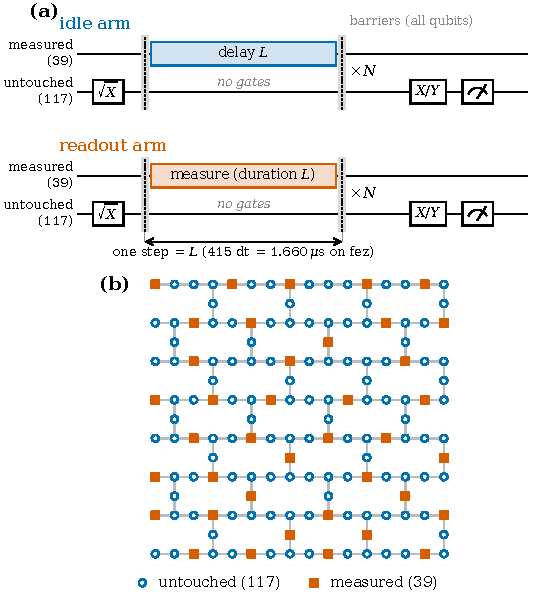
\includegraphics[width=0.98\linewidth]{figures/fig1.pdf}
\caption{Design. (a) One step of each arm, on a shared time axis of exactly the readout length $L$ (1.660\us{} on ibm\_fez). Untouched qubits are prepared on the equator ($\sqrt{X}$), then $N$ steps follow, each bounded by barriers on all qubits. In the idle arm the 39 measured qubits wait $L$; in the readout arm they are measured. Untouched qubits receive no gates during the steps in either arm and are read out at the end in the $X$ or $Y$ basis. (b) Coupling map of ibm\_fez (156 qubits, heavy-hex, cz couplers from the calibration at firing) with the 39 measured qubits (squares) and the 117 untouched qubits (circles); the same roles are used on every processor.}
\label{fig:schematic}
\end{figure}

\paragraph*{Readout against an equal idle, 1 to 25 measured qubits (7 October).} The 32 jobs ran on ibm\_pittsburgh, ibm\_fez, ibm\_aachen and ibm\_kingston. A readout arm of $N$ back-to-back readouts on a measured set and an idle arm of $N$ times the stated length (plain delay, realised on the 16-sample grid within 0.24\% of stated) on the same untouched qubits in the same job; $N\in\{1,2,3,4,6,9\}$ or $\{1,2,4\}$ ($\{2,4\}$ for readouts separated by 3\us{} gaps against a matched idle); 400 shots per circuit; each family run as three jobs (two on aachen). Each untouched qubit is prepared on the equator with a coupled neighbour held in $|1\rangle$ and read on two axes. Families: a corner layout with 12 measured qubits (pittsburgh, fez, aachen); a layout of 25 measured qubits on kingston with the measured qubits in $|0\rangle$, $|1\rangle$ or on the equator, each against an idle in the same state (two runs; the second adds the gapped arms), and the same on pittsburgh; three rotations of the measured and untouched roles (kingston); readout in index and in reversed order after a recalibration (kingston); a whole-chip preparation with measured sets of 20, 19 and 1 qubits (kingston); and two sparse sets of 5 and 7 measured qubits (pittsburgh). No Bell pairs.

\paragraph*{Measured qubit and idle decay (2 to 11 October).} Measured qubits (about 30 per processor) read 1 to 9 times back to back, with idle arms in the same jobs; each qubit's decay from $|1\rangle$ read at 0, 30, 100, 300 and 600\us{} in three copies per job placed by a shuffled circuit order; idle $|0\rangle$ arms at 300 and 600\us. On 11 October, three ibm\_fez jobs read a measured qubit after 1 to 128 readouts with a 40\us{} idle arm in the same jobs. Levels are the raw readout signal projected on the line between the job's own $|0\rangle$ and $|1\rangle$ references (0 and 1 at the references).

\paragraph*{Spaced X-gate trains (2 to 7 October).} Starts $|0\rangle$, $|1\rangle$ or the equator state; ten X gates each preceded by an interval (30\us{} on 2 October; 5 to 150\us{} on 4 October; the per-gate residual also uses runs of 5 to 7 October on boston, aachen and phoenix), or back to back; one readout at the end; all qubits driven and read. The expected level is propagated as a two-state chain in which $|1\rangle$ survives an interval $T$ with probability $q_T$ and each X swaps the levels, with three choices of $q_T$, all per qubit and from the same job: one exponential through the 300\us{} level, each interval's own measured decay, or the job's decay curve (log-linear between 0, 30, 100, 300 and 600\us; an interpolation below 30\us). Excess is measured level minus bookkeeping. On 22 October a gate train with the decay shape held equal compares X~X~X against X on the same waits (2, 6, 10 steps) on fez, kingston, marrakesh and phoenix.

\paragraph*{Second vendor.} On Rigetti Cepheus-1-108Q a qubit (q0) is driven to $|2\rangle$ and a directly coupled neighbour (q9) runs as a Ramsey qubit (28 September and 4 October); on 4 October seven qubits receive ten back-to-back X gates while their 22 neighbours are at rest, driven in step, or held on the equator. There is no readout-against-idle design on this processor.

\subsection{Estimators}

A known-good rule is a pass/fail check, fixed in the plan before the job, that a run's reference arm must meet for its decisions to count; committed means saved to the public repository before the data were read. Every reading of the 21--22 October runs is a difference between two arms of the same job, per qubit or per pair, median over qubits, with a 95\% bootstrap interval (2000 resamples). Phase is $\arctan(\langle Y\rangle/\langle X\rangle)$, unwrapped; the kick per readout is (readout $-$ idle phase)/$N$. Four outcomes are allowed: above 0, below 0, consistent with 0 (the interval is then the bound), or cannot tell (fewer than five units, or the two copies of a circuit disagree). In the 22 October runs copies are compared by their difference (copy gap) and a gap interval excluding 0 is reported as cannot tell; in the 21 October control, raw-readout and pair runs the committed rule was that copies disagree when their outcome labels differ, and a copy-gap reading defined after the data is reported where used. Signs are carried. Processors are combined by inverse variance (sigma taken as the 95\% interval width divided by 3.92), the chip-to-chip $\chi^2$/dof is printed, a processor whose copies shifted is left out, and a combined value is quoted only where $\chi^2$/dof is below 2. A value written with $\pm$ is one standard deviation (one width), and its kind is named in the run's own output file: shot noise (analytic, or the Rigetti per-window rates), a bootstrap of 200 resamples (X-gate trains), the fit (the X-gate shortfall per gate and its count-linear term), the spread of three jobs or three reads (decay exponent, the fez reads), or the spread across qubits (the mean rise in Sec.~\ref{sec:rigetti}, standard error with 6 degrees of freedom). A qubit is unreadable (dead) when its coherence is below five times the shot noise. In the control-run analysis and its successors the $Y$ axis is read with the opposite convention to the 21 October run, so the kick prints negative there; sizes are quoted unless a sign is stated.

The 7 October runs are read with the same functions (median, bootstrap, outcome, copy gap, coupling distance by breadth-first search over the saved coupling edges, dead-qubit guard) applied to IQ (in-phase/quadrature) data: each readout is projected on the job's all-$|0\rangle$ to all-$|1\rangle$ axis and thresholded at 0.5. The per-qubit kick is the slope of the unwrapped readout-minus-idle phase against $N$, through the origin; coherence is read as the slope of readout-minus-idle coherence against $N$ and at $N=4$. The copies are separate jobs minutes to an hour apart (copy 0 = first job, copy 1 = the others pooled), a harsher test than two copies in one job. Untouched qubits are kept if their IQ clouds are separated by more than three widths in every job, they pass the dead-qubit guard, and their coherence is at most 1.25. The sign convention was checked by exact gate algebra and by recomputing the 21 October control-run kingston kick through the same code ($-2.8638^\circ$, agreeing with the committed value to $3\times10^{-6}$ deg; the mapping itself rests on the gate algebra). A mean-projection variant gives the same conclusions.

\subsection{Runs, job counts and pre-registration}

Dates are US Eastern unless marked UTC. Table~\ref{tab:runs} lists every period with IBM jobs from 24 September to 23 October 2026 and the Rigetti tasks used here (3035 were fired in all, 25 September to 5 October; the 1310 of 5 October are not used). No IBM job was found for 8 to 10 or 12 to 20 October on any of our IBM credentials (job lists re-pulled on 23 October from every account and instance, after a 22 October pull that missed 26 jobs). A run enters the evidence for the untouched-qubit readings only if it has a readout arm and an idle arm of equal scheduled length on the same untouched qubits in the same job, reads their phase, coherence or concurrence, and has saved job identifiers and outputs; this rule was written before the earlier runs were inventoried, and every run that passes is reported whatever it shows. Under the rule as written, a run that fails it enters only the timeline with no numbers carried into the readout claims. The measured-qubit, idle-decay, X-gate-train, gate and Rigetti readings of 25 September to 11 October come from such runs; they are reported as separate findings outside that rule, with their own designs, and are defined after the data (the 22 October measured-qubit and extra-gate readings were planned before their jobs). Those readings were chosen from a larger set of exploratory analyses of the same jobs with no program-wide multiplicity correction.

\begin{table*}[!tp]
\caption{Runs by period. Jobs are IBM jobs unless marked tasks. ``Hashed'' means the run scripts were frozen by SHA-256 before the job; ``pushed'' means the plan (and, where stated, circuits and analysis) reached a public server before the first job.}
\label{tab:runs}
\footnotesize
\begin{tabular}{p{2.3cm}p{3.6cm}p{6.3cm}p{4.9cm}}
\toprule
Date (2026) & Processors, jobs & Design & Status for this paper \\
\midrule
24 Sep & fez 3, kingston 4, marrakesh 41 (48) & Single qubits and Bell pairs with and without a mid-circuit readout; correlations; three-box weak measurement & No equal-idle arm on untouched qubits; not used \\
28 Sep & fez 37, kingston 5, marrakesh 23 (65) & Raw IQ of every even qubit after one or two readouts; entangled-pair rounds & Not used \\
25--28 Sep & Rigetti, 563 tasks & Neighbour in $|2\rangle$, Ramsey neighbours & Second-vendor shift (Sec.~\ref{sec:rigetti}) \\
1--2 Oct & kingston, phoenix, pittsburgh, boston (12) & One readout per qubit, every qubit read & Not used \\
2--7 Oct & 7 processors (305): pittsburgh 86, kingston 75, marrakesh 55, aachen 25, boston 24, fez 20, phoenix 20; 63 on 2 Oct (9 more are in the row above), 43 on 4, 26 on 5, 48 on 6, 125 on 7 (US Eastern creation day); three errored, one each on 2, 4 and 6 Oct & Untouched qubits' phase against a fitted precession rate; measured-qubit loss; idle decay; X-gate trains & Hashed; no outcomes stated before the 2 Oct and 4 Oct morning runs. Measured-qubit, decay and X-train readings are not pre-registered. An earlier fitted-rate reading of the kick (ratio $1.0207\pm0.0092$, cannot tell) is superseded by the equal-idle design \\
4 Oct & Rigetti, 680 of 1162 tasks (the 16--17 UTC runs used here; 116 cancelled) & Neighbour in $|2\rangle$; X trains with neighbours in three states & No outcome written before the runs \\
7 Oct (within the 305) & pittsburgh 9, fez 3, aachen 2, kingston 18 (32) & Readout against an equal idle, 1 to 25 measured & Plans with OpenTimestamps files (attestations not verified) naming other readings; this recomputation is not pre-registered \\
11 Oct & fez (3 of 14; the other 11 are a three-box weak-measurement probe-strength sweep, not used here) & Measured qubit after 1 to 128 readouts, 40\us{} idle arm & Not pre-registered \\
21 Oct & fez, kingston, marrakesh, pittsburgh (4; a boston job errored) & 39 measured, $N\in\{0,2,4,8,16\}$, 2000 shots & Plan hashed locally 51\,s before the first job; pittsburgh added with the same plan; kick analysis defined after the data \\
21 Oct & fez, kingston, marrakesh (3) & Coherence and concurrence, $N\in\{0,8,16,32\}$ & Plan hashed locally; primary reading the loss ratio at $N=32$ \\
21 Oct & marrakesh (1) & Bell pairs, $N\in\{0,8,16\}$ & Plan hashed locally before the job, not externally timestamped \\
21 Oct & kingston, marrakesh (2) & Excitation test & Plan hashed locally before the jobs, not externally timestamped; second model after the data \\
21 Oct, 23:01 UTC & fez, kingston, marrakesh (3) & Control run: two shuffled copies per job, 1000 shots per copy per setting (4000 for Bell settings), 1, 10 or 39 read out & Plan and circuits pushed 23:00:47 UTC, first job created 23:01:05; analysis pushed 23:02:19, before any result was opened \\
22 Oct, 01:09 UTC & fez, kingston, marrakesh (3 + 6; a kingston test job at 01:02 UTC, before the plan push, is not used) & Raw-readout coherence run; raw-readout pair run & Plans pushed before the jobs; the pair run's synthetic test was generated 13\,s before its plan commit \\
22 Oct 02:23--02:50 UTC & fez, kingston, marrakesh, phoenix (24) & Distance, count, $|1\rangle$ comparison, restart, gates, neighbour, order, coherence come-back & Plan pushed before the first job \\
22 Oct & fez, phoenix (2) + phoenix (1) & One coupled neighbour in superposition (ZZ scale); flat-beat test & Plans pushed before the jobs; the flat-beat known-good was pushed before its output was opened \\
22 Oct & kingston, marrakesh, fez (3) & Two readout instructions (\texttt{measure}, \texttt{measure\_2}), each against its own equal idle & Plan pushed before the jobs; marrakesh excludes a kick fixed per readout (proportional to length at 4 readouts, outside both at 8), kingston not decided by its known-good (a repeat the same night meets it and reads a kick fixed per readout at 8 readouts), fez cannot tell (known-good met) \\
22 Oct & 3 + 3 + 1 + 6 + 3 + 3 & Echo; reach; kingston repeat of the $|1\rangle$ comparison (4900 shots); pairs repeat; flip checks 1 and 2 & Plan, circuits and analysis pushed before each run's jobs \\
22 Oct & marrakesh (1; a fez job cancelled while queued) & Three-box weak measurement & Plan, analysis and known-good pushed before the job; not used \\
22 Oct & fez (1; ibm\_phoenix not run) & Direct ZZ phase shift per edge & Plan pushed before the job; not read at submission; not used \\
23 Oct & fez, phoenix (2) & Direct ZZ phase shift per edge, second run on the same pairs & Plan, analysis and known-good pushed before the jobs \\
\bottomrule
\end{tabular}
\end{table*}

\section{Results}

\subsection{A phase kick on untouched qubits}\label{sec:kick}

\paragraph*{39 measured qubits.} Each readout (default \texttt{measure} instruction) kicks the phase of untouched qubits by $1.73^\circ$ [1.29, 2.21] (fez), $2.41^\circ$ [1.96, 3.58] (kingston), $2.13^\circ$ [1.44, 2.79] (marrakesh) and $1.79^\circ$ [1.16, 2.66] (pittsburgh) in the 21 October run (median over 117 qubits). The run's planned ratio of readout to idle phase (plan hashed locally) reads 1.17 to 1.20, above 1 on all four processors, the direction an extra readout time would give; it falls to 0.95 to 1.10 with a rate cut and depends on which slowly precessing qubits are kept, so it is not used, and the additive analysis defined after the data is used instead (Sec.~\ref{sec:causes}). The control run gives 1.62, 2.86 and $2.39^\circ$ on fez, kingston and marrakesh, all intervals clear of 0 (Fig.~\ref{fig:kick}), and the echo run's arms without echo give $-1.50$ [$-2.00$, $-0.95$], $-3.24$ [$-3.81$, $-2.04$] and $-2.50^\circ$ [$-3.49$, $-1.76$]. Sizes in this paragraph are magnitudes; with sign, every one is negative in the convention of Fig.~\ref{fig:kick} and Table~\ref{tab:oct07}.

\begin{figure*}[t]
\centering
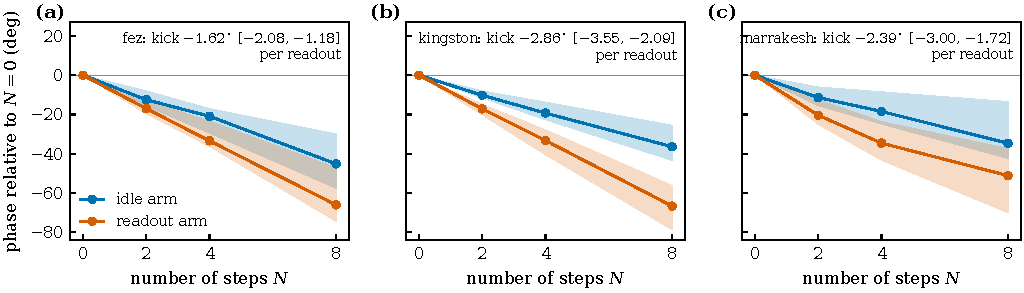
\includegraphics[width=\textwidth]{figures/fig2.pdf}
\caption{Phase of the 117 untouched qubits after $N$ steps, relative to $N=0$, in the idle arm and the readout arm of the same job (control run). Points: median over qubits of the unwrapped per-qubit phase, $\arctan(\langle Y\rangle/\langle X\rangle)$, both copies pooled; bands: 95\% bootstrap intervals (2000 resamples). The kick per readout is (readout $-$ idle phase at $N=8$)/8, median over qubits with 95\% interval, quoted in the text; it is negative in this analysis's $Y$ convention, and the text quotes sizes.}
\label{fig:kick}
\end{figure*}

\paragraph*{Layout and distance.} In the 39-qubit layout every untouched qubit lies within two couplings of a measured one; the median kick over all untouched qubits in the three reach layouts, where most are three or more couplings away, is 0.06 to $0.13^\circ$ per readout (0.056 to 0.125). With the 39 packed in one region (distance run), untouched qubits three to four couplings from the nearest measured one are kicked by 0.81, 1.77 and $1.30^\circ$ per readout (fez, kingston, marrakesh; 15 qubits, every interval above 0); they are not wired to any measured qubit. Within two couplings in the packed layout only kingston is resolved ($3.458^\circ$; 10 qubits; fez copies shifted, marrakesh not resolved), and at five or more couplings (92 qubits) the kick is consistent with zero on all three ($+0.0039$ [$-0.029$, $+0.037$] combined). The reach run (three packed layouts) resolves the kick at 4 couplings with the three processors combined (size $+0.21$ [$+0.09$, $+0.32$]$^\circ$; fez $+0.19$ [$+0.10$, $+0.36$], kingston $+0.13$ [$+0.04$, $+0.69$], marrakesh $+0.40$ [$+0.07$, $+0.77$]) and at 3 couplings on fez ($+0.11$ [$+0.001$, $+0.57$]) and marrakesh ($+0.52$ [$+0.15$, $+1.71$]) singly; kingston at 3 couplings reads $+0.51$ [$-0.005$, $+1.30$] and the three combined $+0.21$ [$-0.04$, $+0.45$], both consistent with zero. At 5 couplings the combined reading is resolved ($+0.055$ [$+0.002$, $+0.108$]) and no processor resolves it alone; 6 couplings and beyond are consistent with zero combined (upper ends 0.03 to $0.06^\circ$), while marrakesh alone reads 6 couplings above zero ($+0.050$ [$+0.002$, $+0.155$]). The committed edge rule names no combined edge; by processor the unbroken edge is 4 couplings on fez and marrakesh and none on kingston. Per-layout medians at the same distance differ several-fold. Readings were not corrected for multiplicity: synthetic runs with no kick resolve 6.0\% of single-processor readings and 5.6\% of combined ones, so the resolutions at 3 couplings on fez, at 5 couplings combined and at 6 couplings on marrakesh, whose lower ends are 0.001 to 0.002, are not distinguished from that floor.

\paragraph*{1 to 25 measured qubits (7 October).} Table~\ref{tab:oct07} gives every arm that passes the inclusion rule, in the convention of Fig.~\ref{fig:kick} (negative is the direction of the 21--22 October kick). On kingston the 14 arms with 25 measured qubits (six from the same three jobs, all on overlapping untouched qubits) read the kick over all untouched qubits below zero in 13 of them ($-0.26$ to $-0.58^\circ$ per readout), with the measured qubits in $|0\rangle$, in $|1\rangle$ or on the equator, back to back or with 3\us{} gaps, in all three role rotations and in index order; within two couplings it is below zero in 12 of 14 arms ($-0.69$ to $-1.38^\circ$, intervals heavy-tailed on the low side). Across Table~\ref{tab:oct07}, 18 of the 25 arms are below zero within two couplings (0.33 to 3.13$^\circ$). The whole-chip measured sets of 20 and 19 qubits give $-0.69$ and $-0.81^\circ$ overall and $-2.84$ and $-3.13^\circ$ within two couplings. In all these arms, at five or more couplings no arm is below zero; the reversed-order arm reads above zero, $+0.175$ [$+0.036$, $+0.311]^\circ$ (15 qubits), the only interval above zero among the 25 arms at five or more couplings; with about 100 distance-bin readings in this table it is not distinguished from the false-reading floor. A single measured qubit (whole-chip preparation, set C) gives $-0.138$ [$-0.309$, $+0.115$], consistent with zero. On pittsburgh the 25-qubit layout is below zero overall in all three states ($-0.22$ to $-0.36^\circ$) and within two couplings ($-0.43$ to $-0.83^\circ$); the sparse sets of 5 and 7 measured qubits are consistent with zero overall and below zero within two couplings for the first set only ($-0.330$ [$-0.813$, $-0.169$]). The corner layout with 12 measured qubits, where 64 to 67 of the 73 to 76 kept untouched qubits are five or more couplings away, is consistent with zero overall on pittsburgh ($+0.000$ [$-0.082$, $+0.061$]), fez ($-0.036$ [$-0.087$, $+0.063$]) and aachen ($+0.008$ [$-0.127$, $+0.150$]), with only four qubits within two couplings (cannot tell). Pooling the plain $|0\rangle$ arms per processor (untouched qubits repeat across families, so $n$ counts repeated measures) gives pittsburgh $-0.136$ [$-0.199$, $-0.063$] overall and $-0.094$ [$-0.147$, $-0.026$] at five or more couplings; the second interval treats repeated measures of the same qubits as independent and is too narrow, and no single pittsburgh family is below zero at five or more couplings; and kingston $-0.433$ [$-0.633$, $-0.221$] overall and $-0.065$ [$-0.284$, $+0.085$] at five or more; the per-family readings are the readings of record. Two arms do not pass the rule and are not read: the corner-layout arms whose readout was the shorter \texttt{measure\_2} instruction (no idle arm of equal length), and a whole-chip arm that prepared only one untouched qubit on the equator. A single-qubit chain on kingston (one untouched qubit, one measured qubit two couplings away) cannot enter a median over qubits (cannot tell). These runs differ from those of 21--22 October in the number of measured qubits, the neighbour held in $|1\rangle$, the number of readouts and the copy test; they are read beside them and never pooled. On kingston, the processor in both, the 7 October overall medians ($-0.26$ to $-0.81^\circ$; 19 to 25 measured, up to 9 readouts) and the 21--22 October medians (2.41 to $3.24^\circ$ in size; 39 measured, every untouched qubit within two couplings) are of the same sign and are not compared as one quantity.

\begin{table*}[!tp]
\caption{Equal-idle runs of 7 October, recomputed with the estimators of this paper. Kick: slope of readout-minus-idle phase against $N$ (degrees per readout; negative is the direction of the 21--22 October kick), median over untouched qubits with 95\% bootstrap interval, by coupling distance $d$ to the nearest measured qubit. Coherence: slope of readout-minus-idle coherence against $N$, all kept qubits (negative is a loss). Outcomes as printed: B below 0, A above 0, C consistent with 0, CT cannot tell (fewer than five qubits, or the jobs disagree). $n$: kept qubits, all / $d\le2$ / $d=3$--4 / $d\ge5$. Processors: P pittsburgh, F fez, Aa aachen, K kingston; 400 shots per circuit, three jobs per family (two on aachen).}
\label{tab:oct07}
\scriptsize
\begin{tabular}{p{3.6cm}p{1.6cm}p{2.15cm}p{2.15cm}p{2.15cm}p{2.15cm}p{2.15cm}}
\toprule
Layout, arm & $n$ & kick, all & kick, $d\le2$ & kick, $d=3$--4 & kick, $d\ge5$ & coherence, all \\
\midrule
P corner, 12 measured & 76/4/5/67 & $+0.000$ C [$-0.082$,$+0.061$] & CT & $+0.036$ C [$-1.911$,$+0.380$] & $+0.003$ C [$-0.082$,$+0.065$] & $-0.000$ C [$-0.001$,$+0.000$] \\
F corner, 12 measured & 73/4/5/64 & $-0.036$ C [$-0.087$,$+0.063$] & CT & $-0.242$ C [$-0.423$,$+0.068$] & $-0.009$ C [$-0.055$,$+0.085$] & $-0.001$ B [$-0.002$,$-0.000$] \\
Aa corner, 12 measured & 75/4/5/66 & $+0.008$ C [$-0.127$,$+0.150$] & CT & $-0.171$ C [$-1.836$,$+0.340$] & $+0.030$ C [$-0.094$,$+0.158$] & CT \\
K 25, measured in $|0\rangle$ & 57/25/17/15 & $-0.323$ B [$-0.622$,$-0.112$] & $-0.734$ B [$-12.857$,$-0.263$] & $-0.384$ B [$-1.096$,$-0.025$] & $-0.096$ C [$-0.267$,$+0.128$] & $-0.000$ C [$-0.001$,$+0.001$] \\
K 25, in $|1\rangle$ & 56/25/16/15 & $-0.257$ B [$-0.692$,$-0.100$] & $-0.692$ B [$-17.486$,$-0.251$] & $-0.650$ B [$-1.450$,$-0.097$] & $-0.066$ C [$-0.124$,$+0.159$] & $-0.001$ B [$-0.001$,$-0.000$] \\
K 25, on the equator & 56/25/16/15 & $-0.302$ B [$-0.527$,$-0.109$] & $-0.846$ B [$-14.930$,$-0.307$] & $-0.146$ C [$-0.722$,$+0.174$] & $-0.106$ C [$-0.287$,$+0.091$] & $-0.000$ C [$-0.001$,$+0.000$] \\
K 25 (2nd run), $|0\rangle$ & 58/25/18/15 & $-0.338$ B [$-0.873$,$-0.052$] & $-1.024$ B [$-12.692$,$-0.161$] & $-0.682$ C [$-1.280$,$+0.445$] & $-0.024$ C [$-0.157$,$+0.204$] & $-0.002$ C [$-0.003$,$+0.000$] \\
K 25 (2nd run), $|1\rangle$ & 58/25/18/15 & $-0.466$ B [$-0.712$,$-0.076$] & $-1.133$ B [$-17.225$,$-0.082$] & $-0.302$ C [$-1.532$,$+0.414$] & CT & $-0.001$ C [$-0.003$,$+0.000$] \\
K 25 (2nd run), equator & 58/25/18/15 & $-0.577$ B [$-1.005$,$-0.298$] & $-1.378$ B [$-13.451$,$-0.346$] & $-0.357$ C [$-1.005$,$+0.047$] & $-0.305$ C [$-0.680$,$+0.001$] & $-0.003$ B [$-0.004$,$-0.001$] \\
K 25, 3\us{} gaps, $|0\rangle$ & 57/25/17/15 & $-0.572$ B [$-1.000$,$-0.114$] & $-1.270$ B [$-12.614$,$-0.602$] & $-0.124$ C [$-1.283$,$+0.281$] & $+0.329$ C [$-0.572$,$+0.647$] & $+0.001$ C [$-0.001$,$+0.002$] \\
K 25, 3\us{} gaps, $|1\rangle$ & 57/25/17/15 & $-0.434$ B [$-0.708$,$-0.186$] & $-0.722$ B [$-12.588$,$-0.351$] & $-0.510$ B [$-1.335$,$-0.117$] & $+0.152$ C [$-0.448$,$+0.435$] & CT \\
K 25, 3\us{} gaps, equator & 57/25/17/15 & $-0.437$ B [$-0.718$,$-0.011$] & $-1.192$ C [$-12.673$,$+0.041$] & $-0.509$ C [$-1.149$,$+0.055$] & $+0.039$ C [$-0.437$,$+0.449$] & $+0.000$ C [$-0.001$,$+0.002$] \\
K 25, role rotation 0 & 58/25/18/15 & $-0.428$ B [$-0.758$,$-0.290$] & $-1.116$ B [$-18.259$,$-0.411$] & $-0.416$ C [$-1.013$,$+0.143$] & $+0.004$ C [$-0.360$,$+0.314$] & $+0.000$ C [$-0.002$,$+0.002$] \\
K 25, role rotation 1 & 58/25/18/15 & $-0.290$ B [$-0.966$,$-0.075$] & $-1.211$ B [$-13.749$,$-0.033$] & $-0.563$ B [$-1.536$,$-0.128$] & $+0.039$ C [$-0.311$,$+0.253$] & CT \\
K 25, role rotation 2 & 58/25/18/15 & $-0.518$ B [$-0.928$,$-0.319$] & $-1.124$ B [$-16.048$,$-0.303$] & $-0.767$ B [$-1.229$,$-0.202$] & $-0.173$ C [$-0.417$,$+0.001$] & $-0.001$ C [$-0.004$,$+0.001$] \\
K 25, index order & 58/25/18/15 & $-0.386$ B [$-0.894$,$-0.144$] & $-1.066$ B [$-13.476$,$-0.489$] & $-0.520$ B [$-1.699$,$-0.083$] & $+0.239$ C [$-0.041$,$+0.524$] & $-0.001$ C [$-0.003$,$+0.001$] \\
K 25, reversed order & 58/25/18/15 & $-0.450$ C [$-0.945$,$+0.064$] & $-1.192$ C [$-12.986$,$+0.019$] & $-0.702$ C [$-1.537$,$+0.068$] & $+0.175$ A [$+0.036$,$+0.311$] & $-0.000$ C [$-0.003$,$+0.001$] \\
K whole chip, set A (20) & 64/20/32/12 & $-0.688$ B [$-1.182$,$-0.345$] & $-2.840$ B [$-5.900$,$-0.515$] & $-0.490$ B [$-0.789$,$-0.062$] & $-0.455$ C [$-1.063$,$+0.133$] & $-0.000$ C [$-0.004$,$+0.002$] \\
K whole chip, set B (19) & 64/18/30/16 & $-0.811$ B [$-1.128$,$-0.214$] & $-3.129$ B [$-5.545$,$-0.449$] & $-0.707$ B [$-1.091$,$-0.214$] & $+0.024$ C [$-1.128$,$+0.229$] & $-0.001$ C [$-0.003$,$+0.002$] \\
K whole chip, set C (1) & 64/3/8/53 & $-0.138$ C [$-0.309$,$+0.115$] & CT & $-0.134$ C [$-0.590$,$+0.431$] & $-0.145$ C [$-0.345$,$+0.130$] & $+0.000$ C [$-0.002$,$+0.001$] \\
P sparse set 0 (5) & 84/15/30/39 & $-0.169$ C [$-0.288$,$+0.015$] & $-0.330$ B [$-0.813$,$-0.169$] & $-0.087$ C [$-0.267$,$+0.274$] & $-0.099$ C [$-0.372$,$+0.118$] & $-0.001$ C [$-0.002$,$+0.000$] \\
P sparse set 1 (7) & 84/15/34/35 & $-0.235$ C [$-0.358$,$+0.017$] & $-0.410$ C [$-0.623$,$+0.111$] & $-0.142$ C [$-0.492$,$+0.147$] & $-0.236$ C [$-0.373$,$+0.041$] & $-0.001$ C [$-0.003$,$+0.001$] \\
P 25, measured in $|0\rangle$ & 58/26/16/16 & $-0.224$ B [$-0.400$,$-0.051$] & $-0.433$ B [$-2.950$,$-0.166$] & $-0.223$ C [$-0.608$,$+0.029$] & $+0.280$ C [$-0.134$,$+0.447$] & CT \\
P 25, in $|1\rangle$ & 58/26/16/16 & $-0.356$ B [$-0.751$,$-0.137$] & $-0.796$ B [$-3.230$,$-0.225$] & $-0.570$ B [$-0.937$,$-0.106$] & $-0.093$ C [$-0.255$,$+0.270$] & CT \\
P 25, on the equator & 59/27/16/16 & $-0.334$ B [$-0.647$,$-0.053$] & $-0.826$ B [$-2.865$,$-0.054$] & $-0.558$ C [$-0.821$,$+0.111$] & $+0.009$ C [$-0.368$,$+0.364$] & $-0.001$ C [$-0.004$,$+0.001$] \\
\bottomrule
\end{tabular}
\end{table*}

\subsection{Causes the kick is not}\label{sec:causes}

\paragraph*{Extra elapsed time.} Extra time would advance each qubit along its own precession, so qubits precessing in opposite directions in the idle arm would be kicked in opposite directions. They are kicked the same way: the 21 to 36 qubits per processor whose idle phase turns opposite to the majority are kicked by 1.0 to $3.4^\circ$ per readout (fez 1.18 and 0.96, kingston 3.03 and 2.80, marrakesh 3.37 and $1.52^\circ$ in the control and raw-readout runs), every interval clear of 0 (Fig.~\ref{fig:controls}a). In the control run (bound defined after the data) the 95\% upper bounds on extra readout time that advances untouched qubits' phase are 4, 1 and 12\% (rounded up from 3.7, 0.8 and 11.4\%; fez, kingston, marrakesh); the bound comes from a slope fit dominated by the minority group, whose backward-minus-forward differences have intervals of $\pm1$ to $2^\circ$.

\paragraph*{Measured qubits in $|1\rangle$.} With an idle arm that also holds the measured qubits in $|1\rangle$, the kick in $|1\rangle$ is $0.18^\circ$ (fez) and $0.92^\circ$ (marrakesh) per readout smaller than in $|0\rangle$ (22 October). On kingston the first 22 October job's kick in $|0\rangle$ had shifted copies (cannot tell) and the difference reads $+0.066$ [$-0.005$, $+0.229$], consistent with zero; the repeat job bounds any increase to about $0.1^\circ$ ($+0.049$ [$-0.098$, $+0.132$], copies agree). In the 21 October excitation test, re-read after the data, the difference (kick in $|1\rangle$ minus kick in $|0\rangle$) is $+0.204$ [$-0.092$, $+0.320$] on kingston (larger in $|1\rangle$ by at most $0.32^\circ$; consistent with zero) and $-0.673$ [$-0.982$, $-0.403$] on marrakesh (smaller in $|1\rangle$); this difference is oriented opposite to Fig.~\ref{fig:controls}b, where a positive value means a smaller kick in $|1\rangle$. The runs are reported beside each other and not combined. Holding the measured qubits in $|1\rangle$ without any readout shifts the untouched qubits' phase by $2.5$ to $3.4^\circ$ per step (22 October: 2.53, 3.24, 3.36 on fez, kingston, marrakesh; 21 October: 3.10 and 3.12 on kingston and marrakesh), which is why the comparison needs the matched idle (Fig.~\ref{fig:controls}b). In the 7 October 25-qubit layouts on kingston and pittsburgh the kick with the measured qubits in $|1\rangle$, each against its own idle in $|1\rangle$, is below zero overall in every arm, with sizes in the range of the $|0\rangle$ arms (Table~\ref{tab:oct07}).

\begin{figure}[t]
\centering
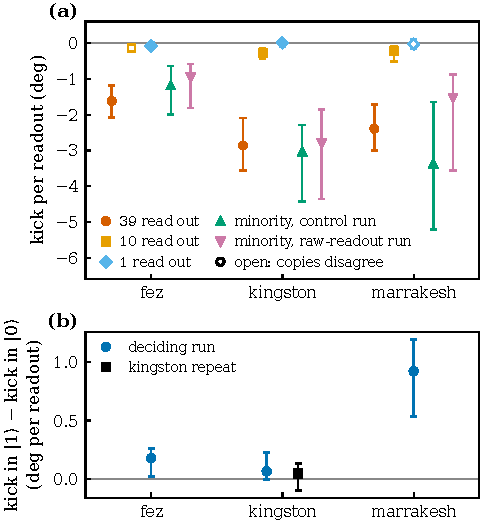
\includegraphics[width=0.98\linewidth]{figures/fig3.pdf}
\caption{Controls on the kick (control run, $N=8$, unless stated). (a) Kick per readout with all 39 measured qubits read out, with 10 and with 1 read out on the same schedule (the rest idling exactly $L$), and for the minority of untouched qubits whose idle phase turns the other way (control and raw-readout runs). (b) Kick with the measured qubits held in $|1\rangle$ minus kick with them in $|0\rangle$, each against an idle in the same state (22 October), and the kingston repeat, shown side by side and not pooled. In this sign convention a positive value means a smaller kick in $|1\rangle$. Medians over 117 untouched qubits, 95\% bootstrap intervals; open markers: the two copies of the circuit disagree.}
\label{fig:controls}
\end{figure}

\paragraph*{Number read out.} On the same schedule, reading out 1 of the 39 qubits leaves at most $0.15^\circ$ on fez and $0.09^\circ$ on kingston (95\% bounds; on marrakesh the copies disagree by the committed rule, and a copy-gap reading defined after the data finds no shift and bounds it at $0.15^\circ$, $-0.029$ [$-0.154$, $+0.100$]); reading out all 39 gives the full kick, and a fixed offset of the full kick is excluded on all three, every copy's interval lying at least 1.4, 2.7 and $2.2^\circ$ from it. Reading out 10 of the 39 gives 0.13, 0.28 and $0.23^\circ$ (8 to 10\% of the full kick, less than the proportional 26\%; fez copies disagree by the committed rule, with no shift by copy gap, pooled $-0.133$ [$-0.226$, $-0.030$], and a repeat on 22 October with the same code reads $-0.167$ [$-0.323$, $-0.068$] with both copies below zero, 11\% of that job's own full kick of $-1.47^\circ$; marrakesh copies read 0.32 and $0.48^\circ$, the pooled median smaller than either), so the kick is not proportional to the number read out. The subsets of 1 and of 10 are one random draw (seed 20261021), and the single qubit is one position. In the control run the kick next to a measured qubit minus two steps away is $-0.612$, $-1.599$ and $+0.332^\circ$ (fez, kingston, marrakesh), resolved on none.

\paragraph*{Growth and wear-out.} The kick after 8 readouts minus after 2 is consistent with 0 ($+0.036$, $-0.008$, $+0.294^\circ$; at most 14, 6 and 24\% of the kick; control and raw-readout runs pooled as printed), and a straight-line intercept is $-0.769^\circ$ on marrakesh. In the restart run (window coherence 0.53 to 0.76, so phases are readable), against 72 equal idles the kick after 72 readouts differs by $+0.028$ [$-0.038$, $+0.085$] (fez), $+0.006$ [$-0.034$, $+0.059$] (kingston) and $-0.036$ [$-0.118$, $+0.104$] (marrakesh) degrees per readout, consistent with zero on all three (the fez 72-idle arm had shifted copies); against no preload fez and kingston read $+0.015$ [$-0.076$, $+0.119$] and $+0.029$ [$-0.019$, $+0.074$] (consistent with zero) and marrakesh reads $0.13^\circ$ less [$-0.21$, $-0.04$] of $2.57^\circ$, with window coherence 0.53 against 0.60. In the count run, readouts 27 to 81 read a smaller kick per readout (0.63, 0.73 and $0.43^\circ$) than readouts 1 to 9 (1.56, 2.82, $2.84^\circ$), but by 54 to 81 readouts 67 to 97 of 117 qubits are below five times the shot noise, so the later readings cannot be interpreted.

\paragraph*{Readout instruction.} Each processor also offers a shorter readout instruction, \texttt{measure\_2}; the 22 October run compares each instruction with its own equal idle in one job (plan pushed before the jobs). On ibm\_marrakesh (1.884 against 2.684\us) the shorter instruction gives 0.58 [0.43, 0.73] and 0.51 [0.36, 0.65] of the longer one's kick at 4 and 8 readouts, so a kick fixed per readout is excluded there; the ratio reads proportional to length at 4 readouts and lies outside both 1 and the length ratio (0.70) at 8. On ibm\_kingston (1.380 against 2.180\us) the ratio is 0.92 [0.77, 1.17] at 4 readouts, but the processor is not decided by the run's known-good rule (copy gap [+0.003, +0.091] at 8); a repeat with the same code the same night meets the known-good and reads 1.01 [0.80, 1.37] at 8 readouts, a kick fixed per readout with the length ratio (0.63) excluded, while at 4 readouts its copies disagree; a second repeat with 2000 shots reads 0.95 [0.75, 1.17] at 4 and 0.98 [0.77, 1.28] at 8 readouts, both copies agreeing and the length ratio excluded at both. On ibm\_fez (1.340 against 1.660\us, length ratio 0.81) the ratios 0.85 [0.71, 1.22] and 0.84 [0.73, 1.15] cannot tell, nor does a repeat with 4000 shots (0.94 [0.80, 1.17] and 0.88 [0.71, 1.10]). The two instructions differ in more than length in IBM's calibration record (the discriminator threshold, and the stated readout error on marrakesh and fez). Table~\ref{tab:causes} collects these tests.

\subsection{Echo}\label{sec:echo}

A symmetric echo (X, X) on the untouched qubits in every step of both arms removes most of the kick: per readout $-1.50$, $-3.24$, $-2.50^\circ$ without the echo and $-0.09$ [$-0.18$, $-0.006$], $+0.45$ [$+0.32$, $+0.56$], $-0.27^\circ$ [$-0.39$, $-0.21$] with it on fez, kingston, marrakesh. With the echo the residual is resolved on all three, including $+0.45$ on kingston, opposite in sign, and is not combined. These runs do not separate a shift during the readout from a control-system phase-frame update. Whether the echo changes the coherence cost cannot be told: no change is resolved at 2, 4 or 8 readouts on fez and marrakesh or at 2 and 4 on kingston (kingston at 8: copies disagree), the far interval ends reach 0.5 to 1.3 times the cost itself, fez at 16 readouts reads a larger cost with the echo ($+0.008$), and the echo changes the idle arm's own coherence with a sign that differs between processors. The closest prior work is the protocol of Hothem et al.\ \cite{Hothem2024}: on the 27-qubit ibmq\_algiers they found that XX dynamical decoupling on idle qubits lowers the layer error rate by about 22\% and the estimated mid-circuit-measurement error by up to 38\%, yet the majority of the measurement-induced crosstalk error remains; without decoupling, the estimated measurement error for 15 qubits is 26 times the prediction from IBM's calibration data. In a surface-code memory on ibm\_phoenix, an XX echo on data qubits during ancilla readout lowers the per-round logical error rate of the X-basis memory by 21 and 38\% on two placements (Z memory unchanged within error; ibm\_phoenix is a Nighthawk r2 processor), in a circuit that also uses short readout and fused measurement and reset \cite{Kan2026}; the same study's appendix tracks the phase of the four data qubits next to one ancilla that is delayed in $|0\rangle$ or $|1\rangle$ or read out in $|1\rangle$, reads the state-dependent slope (0.079\,rad/\textmu s) as consistent with a contribution from residual $ZZ$, and reads the dependence on the readout and reset instruction as the time the ancilla spends excited, while our readout-minus-idle difference is taken in the same state, is not larger in $|1\rangle$, and is mapped to three or four couplings. Here the echo is applied in both arms, and phase and coherence are read separately per processor.

\begin{table*}[!tp]
\caption{Ordinary causes of the phase kick on untouched qubits and the test applied to each. Sizes in degrees per readout; sources in Secs.~\ref{sec:kick}--\ref{sec:echo}. Causes of the coherence cost are tested in Sec.~\ref{sec:supcost}.}
\label{tab:causes}
\footnotesize
\begin{tabular}{p{3.6cm}p{6.4cm}p{6.6cm}}
\toprule
Candidate cause & Test & Outcome \\
\midrule
Extra elapsed time (a readout longer than stated) & Qubits whose idle phase turns opposite to the majority; slope bound on extra time & Kicked the same way (1.0 to 3.4); extra time at most 4, 1 and 12\% (fez, kingston, marrakesh; bound defined after the data) \\
State of the measured qubits & Measured qubits in $|1\rangle$, each arm against an idle in $|1\rangle$ & Not larger in $|1\rangle$: 0.18 and 0.92 smaller (fez, marrakesh); kingston: first job cannot tell, repeat job larger by at most about 0.1, 21 October test at most 0.32 \\
A dose proportional to the number read & 1, 10 and 39 of the 39 read on the same schedule & 1 read: at most 0.15 (fez, and marrakesh by copy gap after the data), 0.09 (kingston); a fixed offset of the full kick excluded on all three; 10 read: 8 to 10\% of the full kick pooled (11\% in a fez repeat; upper interval ends 14 to 21\%) against 26\% proportional (fez copies disagree by the committed rule, no shift by copy gap) \\
Direct wiring to a measured qubit & Measured qubits packed in one region & 0.81 to 1.77 at 3 to 4 couplings from the nearest measured qubit, on qubits wired to none \\
Accumulation (wear-out) & 72 readouts against 72 equal idles & Consistent with zero on all three processors (fez 72-idle arm had shifted copies) \\
A phase that a refocusing pulse cannot undo & Symmetric echo (X, X) in both arms & Mostly removed: $-1.50 \to -0.09$, $-3.24 \to +0.45$, $-2.50 \to -0.27$; residual resolved on all three \\
The readout instruction (length and pulse) & \texttt{measure} against \texttt{measure\_2}, each with its own equal idle, same job & Depends on the instruction on ibm\_marrakesh: the shorter instruction (1.884 against 2.684\us) gives 0.58 [0.43, 0.73] and 0.51 [0.36, 0.65] of the longer one's kick at 4 and 8 readouts, so a kick fixed per readout is excluded there. Kingston (1.380 against 2.180\us): 0.92 [0.77, 1.17] at 4 readouts, not decided by its known-good rule (copy gap [+0.003, +0.091] at 8); repeats read 1.01 [0.80, 1.37] at 8, then 0.95 [0.75, 1.17] and 0.98 [0.77, 1.28] at 4 and 8, fixed per readout. Fez (1.340 against 1.660\us): 0.85 and 0.84, cannot tell, also at 4000 shots (0.94, 0.88). The instructions also differ in the discriminator threshold (all three) and the stated readout error (marrakesh, fez) \\
\bottomrule
\end{tabular}
\end{table*}

\subsection{Coherence cost}\label{sec:supcost}

\paragraph*{Raw-readout run.} The median untouched qubit next to a measured one keeps less coherence after readouts than after the same idle. Keeping only shots in which every measured neighbour was verified in its $|0\rangle$ cluster on every readout (97 to 99\% of shots), the cost is $+0.0056$ and $+0.0062$ on kingston and $+0.0087$ and $+0.0205$ on marrakesh after 4 and 8 readouts, all above zero when the copies are pooled (kingston at 4 readouts: neither copy alone resolves it). The committed rule reads kingston and marrakesh at 2 readouts and fez at 2 and 4 as cannot tell, their copies disagreeing; a copy-gap reading defined after the data finds no shift on any of them, and the pooled readings are above zero: $+0.0054$ (kingston) and $+0.0074$ (marrakesh) at 2, fez $+0.0042$ at 2 (at 4, $+0.0057$ by this reading, but $+0.0037$ $[-0.0001, +0.0100]$, consistent with zero, once readout assignment error is corrected, a re-reading by an outside referee (an AI reviewer agent) defined after the data); at 8 readouts it is consistent with zero (Fig.~\ref{fig:cost}a--c). Mid-circuit readouts outside both the $|0\rangle$ and $|1\rangle$ clusters are 0.2 to 0.4\% (fez, kingston) and 1.8\% (marrakesh).

\paragraph*{Other runs of the same processors.} In the 21 October superposition run the readout-minus-idle coherence at 8 readouts is below zero on all three processors, fez $-0.011$, kingston $-0.005$, marrakesh $-0.013$ (intervals below 0), and at 32 readouts $-0.010$, $-0.006$, $-0.014$ with intervals reaching 0; its planned loss ratio at $N=32$ is consistent with 1 on all three (1.011, 1.009, 1.018), a ratio shrinking a deficit toward 1 once the idle loss is large. The control run's pre-registered coherence reading over all 117 untouched qubits, with no selection, gives readout minus idle below zero on kingston at 2 and 4 readouts ($-0.0094$, $-0.0066$; at 8 the copies disagree) and on marrakesh at 2 and 8 ($-0.0108$, $-0.0164$; at 4 the copies disagree), and on fez consistent with zero at 2 and 4 (at 8 the copies disagree); where the copies disagree, a copy-gap reading defined after the data finds no shift, and the pooled readings are $-0.0067$ [$-0.0144$, $+0.0015$] (kingston at 8, consistent with zero), $-0.0107$ [$-0.0168$, $-0.0062$] (marrakesh at 4, below) and $-0.0061$ [$-0.0131$, $-0.0019$] (fez at 8, below); its pre-registered growth slope over 2 to 8 readouts is below zero on marrakesh ($-0.0015$ per readout), consistent with zero on kingston and cannot tell on fez (copies disagree). In the control run the cost after 8 readouts minus after 2 is $+0.0043$ on fez and $+0.0120$ on marrakesh (above zero) and $+0.0047$ on kingston (not resolved); the 31 untouched qubits per processor with no measured neighbour show no resolved coherence loss. In the excitation test the marrakesh qubits with no measured neighbour (31) read $+0.010$ [0.000, 0.019] and the kingston ones $+0.009$ [$-0.006$, 0.018]. In the 7 October runs (1 to 25 measured, at most 9 readouts) the coherence slope over all untouched qubits is below zero in 3 of 25 arms (fez corner, $-0.0008$ per readout; kingston 25 in $|1\rangle$; kingston second run on the equator), cannot tell in 5 and consistent with zero in 17; at $N=4$ it is below zero on aachen ($-0.010$ [$-0.015$, $-0.003$]), in the kingston equator arm ($-0.007$) and in the pittsburgh $|1\rangle$ arm ($-0.009$). Other distance bins and the $N=4$ reading add further below-zero readings and one above-zero reading; the aachen $N=4$ reading sits beside a slope whose copies shifted. These runs resolve a coherence cost in only 3 of 25 arms; at 4 readouts 20 of the 22 arms with a reading have negative medians (arms share qubits, so these are not independent).

\paragraph*{One coupled neighbour in superposition.} With one neighbour of an untouched qubit on the equator and its other neighbours in $|0\rangle$, the untouched qubit's coherence beats at a rate fitted as a scale $s$ times IBM's calibrated static ZZ for that pair (22 October; the plan named $s=1$ and $s=0.5$ before the jobs, the latter from earlier ibm\_phoenix data). On ibm\_fez (32 triples) $s=0.916$ [0.869, 0.983] and 0.981 [0.938, 1.005] for the two neighbours. The fit reads low by construction on fez: a simulation on fez's own triples, calibration and time grid with the scale set to 1 returns 0.875 to 0.908 (three seeds; an outside referee's simulation run through the committed analysis), so both fez values are consistent with $s=1$ (the phoenix-geometry simulation returns 0.995 at $s=1$ and 0.4875 at $s=0.5$). On ibm\_phoenix (20 and 21 triples) $s=0.514$ [0.456, 0.673] and 0.420 [0.303, 0.558], below 1 and, for the first, consistent with 0.5; the two processors differ by $+0.40$ [$+0.28$, $+0.52$]. A run on 37 further phoenix pairs, with fit and analysis fixed before the job, finds the beat does not scale with the calibrated zz: log-log slope 0.19 [0.01, 0.38] by pair ([0.00, 0.37] by triple in an outside referee's recomputation, not in the committed output), against 1.00 [0.89, 1.14] for the same fit on fez; beats of 4 to 23\,kHz (median 12.9) for calibrated values of 11.6 to 58.8\,kHz (the 37 fitted pairs; three further edges calibrated as 0 were not fitted in the committed output); the committed fit applied to those three edges after the data gives 13.9, 15.2 and 10.1\,kHz (copies agree), where IBM's records of 5 and 6 October gave them 17.5, 14.1 and 13.7\,kHz. A single convention factor would leave the slope near 1 (an outside referee's simulation on the same time grid gives 1.05 for a factor of two), so it does not account for the difference. The run's own prediction of no dependence (slope 0) was not met by the pair bootstrap (rank correlation 0.39 [0.05, 0.66]); the referee's triple interval reaches 0.00. A second run on the same 20 triples (23 October), with plan, analysis and a known-good rule on ibm\_fez fixed before the job, reads the shift directly from a Ramsey phase with the neighbour in $|0\rangle$ and then in $|1\rangle$, without a beat fit. On fez it tracks the calibrated zz (log-log slope 0.92 [0.83, 1.02], median shift 1.04 [1.02, 1.08] of the calibrated value, 66 edges). On phoenix it does not: slope $-0.06$ [$-0.63$, 0.32] and median 0.49 [0.45, 0.53] of the calibrated value over the 37 pairs, copies agree. Two phoenix edges (qubit 41) have phase fits that slipped a wrap (residual 1.6 and 1.3\,rad, median 0.08); a residual rule defined after the data, applied to both processors, removes them and two fez edges and gives 0.19 [0.04, 0.37] on phoenix and 0.94 [0.86, 1.03] on fez. The three phoenix edges calibrated as 0 shift by 14.2, 15.4 and 10.2\,kHz (copies agree). The 22 October runs also read the coherence 58 to 78\us{} after preparation against 26 to 50\us{}: with the neighbour on the equator it comes back on ibm\_phoenix ($+0.039$ [$+0.020$, $+0.046$], $n=60$) and keeps falling on ibm\_fez ($-0.168$ [$-0.204$, $-0.086$], $n=92$); neighbour on the equator minus neighbour in $|0\rangle$ is $+0.243$ [$+0.211$, $+0.263$] on phoenix and $+0.002$ [$-0.017$, $+0.025$] on fez. The two processors disagree, so no combined value is quoted.

\paragraph*{Excitation of the measured qubits.} The excitation test (21 October, marrakesh and kingston; plan hashed locally) predicted the readout excess as excitation rate times the coherence cost of a neighbour held fully in $|1\rangle$. A neighbour held in $|1\rangle$ applies a fixed phase, which coherence does not register, so that prediction is zero by construction. The committed output reads the kingston excess as cannot tell and the marrakesh excess as above the prediction; because the prediction is zero by construction, neither reading tests excitation. A second model, defined after the data, lets a neighbour excited only in some shots apply its phase in those shots. With excitation rates measured from the recorded readouts (4.8\% on marrakesh, 3.1\% on kingston; they include readout misassignment, and one kingston measured qubit read 1 in 75\% of shots), the coherence excess after 8 readouts next to a measured qubit is $+0.025$ [0.012, 0.036] on marrakesh against $+0.0008$ from random excitation; on kingston it is $+0.004$ [$-0.003$, 0.014] against $+0.0005$, an interval that contains both 0 and the raw-readout run's kingston cost. In the control run, removing shots with a measured neighbour read as 1 leaves the loss where it was resolved (fez 2 and 8 readouts, kingston 2 and 4, marrakesh all three); a worst-case bound on neighbours that are excited and misread as 0 (0.4 to 1.1\% of shots stuck in $|1\rangle$, acting through a phase) does not exclude them as the whole cost.

\paragraph*{Extra time as the cause.} Two checks in the control run bear on it. The extra-time bound excludes it on kingston (2 and 4 readouts) and does not exclude it on fez and marrakesh; the comparison of 39 read out with 1 read out (the loss with 1 read out is consistent with zero on all three) excludes it on fez ($+0.010$) and marrakesh ($+0.012$) and cannot tell on kingston.

\begin{figure*}[t]
\centering
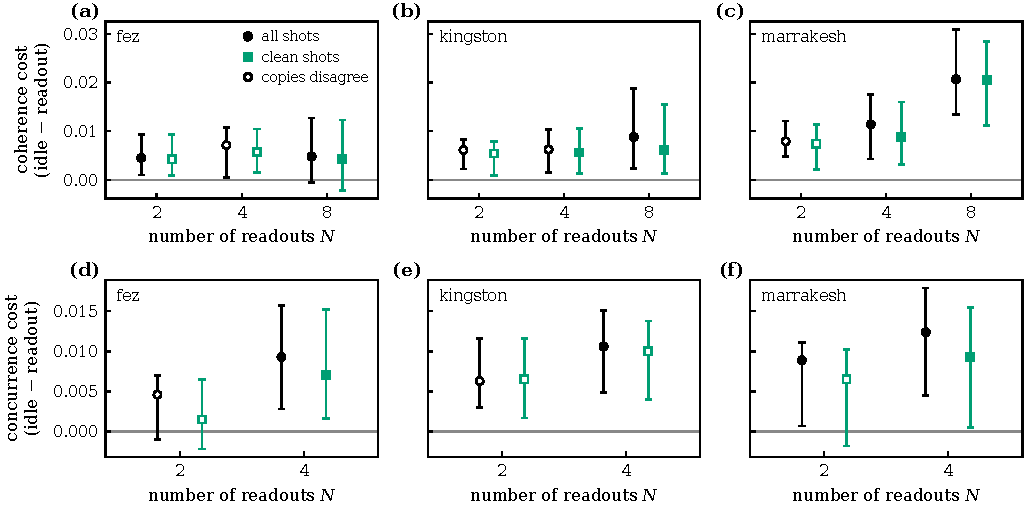
\includegraphics[width=\textwidth]{figures/fig4.pdf}
\caption{Cost of the readouts to untouched qubits, idle minus readout, with all shots and with only shots in which every measured neighbour was verified in its $|0\rangle$ cluster on every readout (97 to 99\% of shots kept). (a--c) Coherence $|\langle X\rangle+i\langle Y\rangle|$ of the 86 untouched qubits wired to a measured qubit (raw-readout run), $N=2,4,8$. (d--f) Concurrence of the X part of untouched Bell pairs (wired, idle concurrence above 0; pair run), $N=2,4$. Medians with 95\% bootstrap intervals, both copies pooled; open markers: the two copies disagree.}
\label{fig:cost}
\end{figure*}

\subsection{Concurrence cost}

The X part of untouched Bell pairs keeps 0.005 to 0.009 less concurrence than after the same idle after 4 readouts on fez and marrakesh, in shots where every measured neighbour was verified in $|0\rangle$ (pairs whose idle concurrence is above 0; this selection can bias the loss upward, and the 39-minus-1 difference, which applies it to both arms, is the unbiased reading). This is resolved on fez ($+0.0051$ [$+0.0005$, $+0.0126$] in the 22 October repeat; $+0.0070$ in the 21 October pair run, 22 October 01:15 to 01:30 UTC) and marrakesh ($+0.0094$ [$+0.0037$, $+0.0243$]; $+0.0093$), in two independent runs each read side by side and never pooled, and on marrakesh also with the pairs wired to three poorly read measured qubits removed. On kingston the committed rule reads the clean-shot reading as cannot tell in either run (copies disagree); a copy-gap reading defined after the data finds no shift in either, and the pooled readings are above zero, $+0.0100$ [$+0.0040$, $+0.0138$] and $+0.0068$ [$+0.0010$, $+0.0170$]; the all-shot reading is above zero in both. The control run's pre-registered concurrence reading over all shots is below zero (a lower value) on all three processors: kingston $-0.0108$ and $-0.0103$ at 2 and 4 readouts, marrakesh $-0.0087$ and $-0.0159$, and fez $-0.0052$ at 4 (consistent with zero at 2). In the control run's selection (every measured neighbour read 0 on every readout) the marrakesh cost is consistent with zero at 2 and 4 readouts ($+0.0060$ [$-0.0020$, $+0.0115$], $+0.0056$ [$-0.0017$, $+0.0181$]), while fez reads $+0.004$ at 4 and kingston $+0.010$ and $+0.009$ at 2 and 4, above zero. In the 21 October pair run the fall in X-part concurrence with 39 qubits read out exceeds the fall with 1 read out by 0.0088, 0.0104 and 0.0065 (marrakesh, kingston, fez; fez a cannot-tell by the committed rule, with no shift by a copy-gap reading defined after the data, $+0.0065$ [$+0.0032$, $+0.0107$]); in the repeat that difference is above zero on kingston and marrakesh and consistent with zero on fez. A time shift per step that is the same whatever number of qubits is read is therefore excluded on kingston and marrakesh in the 21 October run (on fez only by a copy-gap reading defined after the data) and on kingston and marrakesh in the repeat (Fig.~\ref{fig:cost}d--f). A Bell-pair run on marrakesh (plan hashed locally) with $N=0$, 8, 16 lost almost all concurrence by 8 steps in both arms (median 0.79 at the start, 0.08 after 8 idles, 0.065 after 8 readouts, 0 after 16) and cannot tell. These readings are differences of the X-part concurrence between arms and do not bound the change in the pairs' concurrence in either direction.

\subsection{The measured qubit}\label{sec:measured}

On ibm\_fez a qubit that is read out loses more than idling does; on six further processors this follows under an approximate one-exponential conversion (below), which by the decay-shape reading probably overstates the idle-equivalent, so no loss beyond an idle is claimed there without an equal-time comparison; on ibm\_marrakesh and ibm\_kingston the 22 October run gives one (below). At equal elapsed time, with no assumption about the shape of the decay curve, the record holds the comparison on ibm\_fez (11 October, three jobs, a measured qubit prepared in $|1\rangle$, 30-qubit average): 24 readouts (39.8\us{} at the stated length; were the readouts 12\% longer than stated, the idle arm would still read 0.60 to 0.63) leave a signal of 0.517, 0.481 and 0.498, where 40\us{} of idle in the same jobs leaves 0.661, 0.623 and 0.647; at 6 readouts (10.0\us) against 10\us{} of idle the pairs are 0.826 against 0.879, 0.799 against 0.853 and 0.816 against 0.874, and at 12 readouts (19.9\us) 0.694 against 0.796, 0.669 against 0.752 and 0.677 against 0.781. Under repeated readout the signal falls to one half after 22.6 to 25.5 readouts and follows a stretched exponential (exponent $0.823\pm0.012$, $\chi^2$/dof 0.72, 1.38, 1.32). In the 22 October readout-instruction run (pre-registered, a measured qubit prepared in $|1\rangle$, 39 measured qubits, each instruction against its own equal idle), idle minus readout in $P(1)$ after 8 readouts is $+0.038$ [0.032, 0.052] (\texttt{measure}) and $+0.031$ [0.024, 0.038] (\texttt{measure\_2}) on fez and $+0.051$ [0.031, 0.076] and $+0.038$ [0.020, 0.047] on marrakesh, above 0 at 4 readouts as well; on kingston, in a repeat that meets the known-good rule, $+0.063$ [0.050, 0.075] and $+0.035$ [0.023, 0.050].

Converted into idle time on a single-exponential curve, which these qubits do not follow, so that the conversion is approximate, a measured qubit loses per readout what idling 1.5 to 1.7 stated readout lengths would cost it on fez, kingston and marrakesh, and 1.3 to 1.4 on pittsburgh, boston, phoenix and aachen (4 to 6 October, per-processor means of three reads of about 30 measured qubits; single reads 1.2 to 1.8). Two estimators (from blocks of 3 and 9 readouts, and from a fit over 1 to 9) give kingston 1.661 and 1.677, marrakesh 1.516 and 1.509, fez 1.540 and 1.600, pittsburgh 1.340 and 1.360, boston 1.348 and 1.333, phoenix 1.351 and 1.323, aachen 1.371 and 1.351; on fez the three reads spread by $\pm0.224$. The closest members of the two groups differ by 0.14, less than the read-to-read spread on fez; no ordering is claimed. Against the 4, 1 and 12\% bounds on extra readout time for untouched qubits (Sec.~\ref{sec:causes}), 50 to 70\% (30 to 40\% on the other four processors) would be needed to explain this loss as a longer readout.

\subsection{Idle decay: shape, the $|0\rangle$ offset and repeatability}\label{sec:decay}

\paragraph*{Shape.} Idle qubits do not decay along a single exponential. On six processors (26 jobs, 4 to 7 October), 62 to 85\% of qubit-copies prepared in $|1\rangle$ read below the line from their own 300\us{} level at 30\us{} (fez 83.6 to 85.3\%, marrakesh 80.2 to 84.1\%, kingston 72.4 to 77.9\%, boston 63.2 to 71.5\%, aachen 63.9 to 65.1\%, pittsburgh 62.4 to 64.7\%), where a pure exponential passed through the same normalisation, with the same shots and noise, gives 49 to 54\%. The test cannot separate a non-exponential decay from a per-qubit systematic common to the three copies (for example a timing difference between the reference circuit and the idle circuit). In one 2 October ibm\_pittsburgh job (150 qubits) the $|1\rangle$ idle levels are 0.9463, 0.8609, 0.6846 and 0.3286 after 10, 30, 90 and 300\us, the first three $-0.0141$, $-0.0259$ and $-0.0185$ (means of per-qubit deviations) below the exponential through the 300\us{} point. This is the shape expected when the relaxation rate fluctuates from shot to shot through TLS defects \cite{Klimov2018,Schlor2019,Burnett2019,Carroll2022,Muller2019}; these data do not identify the cause.

\paragraph*{The $|0\rangle$ offset.} A qubit prepared in $|0\rangle$ and read after a 300\us{} idle sits 0.04 to 0.80\% above its own job's zero-wait $|0\rangle$ level, above it in all 26 jobs on six processors (marrakesh $+0.80$, $+0.57$, $+0.66\%$; kingston $+0.63$, $+0.37$, $+0.46\%$; pittsburgh $+0.04$ to $+0.32\%$; five of the 26 under two widths, the smallest, $+0.04\%$, at 0.3 widths); at 600\us{} three jobs are at or below zero, so the offset does not grow but is not constant. In three ibm\_pittsburgh jobs a qubit started in $|1\rangle$ and flipped by X gates so that it spends alternate intervals in $|0\rangle$ reads $+0.0017\pm0.0013$, $+0.0020\pm0.0014$ and $+0.0014\pm0.0014$ against its own decay bookkeeping (two halves, quarters or tenths of 300\us{} in $|0\rangle$ alternately; one processor, one day).

\paragraph*{Repeatability.} Repeated measurements of a qubit's decay time (median over the chip, three copies per job) give 168 to 183\us{} on marrakesh, 260 to 270\us{} on kingston (4 October, three jobs each) and 294 to 297\us{} in the first of three pittsburgh jobs (293.8 to 305.5\us{} over all three), and differ by up to 9.8\us{} between jobs and 11.5\us{} between copies inside one job. Compared like with like, the range of three copies in a job is inside the simulated 95th percentile of shot noise alone in 8 of 9 jobs (marrakesh job 301: 10.4 against 8.9\us); the simulation takes its noise scale from the copies themselves, so it cannot separate shot noise from drift between copies.

\subsection{Spaced X-gate trains and the decay-bookkeeping control}\label{sec:xtrain}

A qubit prepared in $|0\rangle$ and given ten X gates spread over 300\us{} (30\us{} intervals) ends above one-exponential bookkeeping (2 October): $+0.0200\pm0.0016$ on pittsburgh (3 jobs; a fourth job read $+0.0126\pm0.0032$, about two widths apart), $+0.0274\pm0.0028$ on marrakesh and $+0.0287\pm0.0028$ on kingston (one job each); started in $|1\rangle$ it reads $+0.0005\pm0.0013$, $-0.0016\pm0.0021$ and $-0.0124\pm0.0024$. With the interval swept (4 October, three jobs on each processor) the start-$|0\rangle$ excess against one exponential is $+0.0302\pm0.0020$, $+0.0325\pm0.0019$ and $+0.0203\pm0.0017$ at 30\us{} (marrakesh, kingston, pittsburgh), grows to $+0.0575$, $+0.0576$ and $+0.0337$ at 5\us, and is $-0.0003$, $+0.0058$ and $+0.0031$ at 150\us; start $|1\rangle$ moves the other way by 31 to 94\% as much at 5 to 20\us{} (against one exponential). The excess does not follow the gate error: in the 4 October runs ten back-to-back gates move starts $|0\rangle$ and $|1\rangle$ by $+1.0$ to $+1.2\%$ and $-1.0$ to $-1.1\%$ on all three processors, and on 2 October marrakesh has a smaller back-to-back shift than pittsburgh ($\pm0.0148$ against $\pm0.023$) and a larger spaced excess ($+0.0274$ against $+0.0200$; one marrakesh job; the difference in excess is $0.0074\pm0.0032$, and pittsburgh's own back-to-back shift was $+0.010$ and $-0.011$ on 4 October). Relaxation toward a thermal population and an imperfect X gate act on the population as maps that do not depend on the start and cannot produce an excess on start $|0\rangle$ alone, and the population in the band where a $|2\rangle$ level at mid-line would read is flat across arms.

Against each job's own decay curve the excess is within $\pm0.007$ on kingston and pittsburgh at intervals of 30\us{} and longer (20\us{}, below the curve's 30\us{} point, is interpolated), and on marrakesh it reverses sign by $-0.012$ to $-0.018$ (start $|0\rangle$) and by up to $-0.016$ (start $|1\rangle$). The bookkeeping therefore removes most of the excess and over-corrects on marrakesh. Most of the excess is a property of the one-exponential bookkeeping, of the size by which the decay right after preparation is faster than one exponential (Sec.~\ref{sec:decay}). At 5 and 10\us{} a residual remains for start $|0\rangle$: $+0.0191$ and $+0.0040$ (marrakesh), $+0.0337$ and $+0.0195$ (kingston), $+0.0157$ and $+0.0096$ (pittsburgh), with the opposite sign for start $|1\rangle$; there the curve is interpolated between its 0 and 30\us{} points, so these runs cannot tell whether that residual is physical.

\subsection{Gate cost against the stated error}\label{sec:gate}

\paragraph*{Per-gate residual.} Against each interval's own measured decay, the start-$|0\rangle$ residual after 2, 6 and 10 spaced gates falls with the number of gates, by $-0.00182$ per gate on fez, $-0.00198$ (first day) and $-0.00136$ (second day, mean of three jobs) on kingston, $-0.00139$, $-0.00154$, $-0.00080$ and $-0.00063$ on boston, and $-0.00107$ on pittsburgh: $-0.0006$ to $-0.0020$ on four processors (pittsburgh from one run at about two shot-noise widths, its per-qubit share cannot tell, $p=0.06$), with 58 to 70\% of individual qubits negative on fez, kingston and boston (54 to 62\% on aachen), and about zero on phoenix on its second day ($-0.00002$; $-0.00058\pm0.00029$ on the first; square lattice). The sign is negative in 9 of 9 runs on fez, kingston and boston (three processors) under all three bookkeepings, and in 11 of 12 when aachen is added. Simulated perfect X gates with a decay rate that varies from shot to shot and persists through a circuit reproduce it (the rate-spread width fitted per run to the share of qubits below the 300\us{} extrapolation; model $-0.00177$ against measured $-0.00136$, mean of nine runs, ratio 1.30), while a stretched exponential restarted at each X and a rate spread redrawn at every wait do not ($+0.00015$ each). With the decay shape held equal (X~X~X against X on the same waits, 22 October) an extra X gate costs $0.0001643$ [$0.00005906$, $0.0002695$] combined over fez, kingston, marrakesh and phoenix, and its difference from IBM's stated X error is $-0.0002279$ [$-0.0003419$, $-0.0001139$]; the train does not see everything the stated error includes, so this is not a claim that the gates are better than stated. On fez and kingston, where both were measured, the residual is opposite in sign to the extra-gate cost and at least twice its upper edge (0.00027), so it is not a gate cost there; no extra-gate test exists on boston or pittsburgh.

\paragraph*{Back-to-back gates.} From back-to-back trains on pittsburgh (2 October, three jobs), ten gates shift starts $|0\rangle$ and $|1\rangle$ by $+2.29$ and $-2.32\%$; the X gate falls $1.47\pm0.12^\circ$ short of a half turn, and a term growing linearly with the gate count ($b$ in a fitted shift $N^2\epsilon^2/4+Nb$ after $N$ gates, $\epsilon$ the shortfall) gives $4b=0.261\%$ per gate (width 0.104\%, upper edge at two widths 0.47\%). This term is a measured value that covers every error growing with the gate count (leakage, decay during the pulse, pulse noise), not leakage alone. The shortfall alone predicts the equator start's loss: $0.026\pm0.002$ for two gates (measured 0.0262) and $0.127\pm0.010$ for ten (measured 0.114).

\paragraph*{Neighbours and order.} A neighbour in superposition does not raise gate error (error with neighbours in $|+\rangle$ over neighbours in $|0\rangle$: 1.000, 0.995, 0.999 on fez, kingston, marrakesh), a neighbour in $|1\rangle$ rather than $|0\rangle$ lowers it slightly ($-0.0000162$ [$-0.0000305$, $-0.0000019$] combined), and the excited population of each read slot is the same across orders (every combined slot interval inside $\pm0.00018$; per processor up to $\pm0.00033$, kingston slot 1 copies shifted). Reading all qubits together rather than one alone raises it by $+0.000166$ [$+0.000025$, $+0.000306$] (three processors combined; each processor's interval touches zero), and the qubit read last sits below the qubit read first on marrakesh ($-0.000375$ [$-0.0005$, $-0.000167$]; fez and kingston include zero, and the chip-to-chip $\chi^2$/dof is 3.05, so no combined value is quoted). These single-processor labels are sensitive to the bootstrap seed (Sec.~\ref{sec:controls}).

\subsection{Second vendor: a neighbour in $|2\rangle$}\label{sec:rigetti}

On Rigetti Cepheus-1-108Q, with a directly coupled neighbour (q0) prepared in $|2\rangle$, the precession rate of a Ramsey qubit (q9) shifts by $-54.93\pm1.28^\circ$/\textmu s on 28 September and $-38.64\pm1.62^\circ$/\textmu s on 4 October (windows 0.5 to 2\us, inverse-variance mean of per-window rates, shot noise only; ratio 0.70; the dates differ by $16.3\pm2.1^\circ$/\textmu s, and on 28 September the per-window rates are not constant, $\chi^2$/dof 9.6). The pair is the same on both dates; between them the $|1\rangle$--$|2\rangle$ pulse amplitude was retuned, the number of simultaneous Ramsey qubits changed from 1 to 106, and the processor was recalibrated, so the difference is not assigned to the coupling. With q0 in $|1\rangle$, q9 moves by $+0.5$, $+5.9$ and $+1.7^\circ$/\textmu s at 0.5, 1 and 2\us; the other coupled neighbour (q1) moves by $-27.5$, $-19.4$ and $-21.0^\circ$/\textmu s with q0 in $|2\rangle$; 101 qubits three or more links from q0 read a median of $+1.06^\circ$/\textmu s (quartiles $-1.9$ to $+2.9$) at 1\us. Over 22 other pairs of a qubit in $|2\rangle$ and a coupled neighbour (4 October, 1\us{} window) the shift spans $-72.8$ to $+30.9^\circ$/\textmu s (median $-6.4$): on this processor sign and size are properties of the pair.

On the same processor, seven qubits given ten back-to-back X gates read 1 more often when their 22 neighbours are held on the equator around the train (read-1 fraction 0.1102, 0.1010 and 0.1038 in three rounds) than at rest (0.0643, 0.0641, 0.0584); the mean rise is $+0.0427\pm0.0182$ over the seven qubits ($t=2.34$ on 6 degrees of freedom, below the 2.447 critical value). In that arm the neighbours end in $|1\rangle$ at the readout (about 94\%), and readouts are correlated between neighbours even at rest, so neighbours on the equator during the train and neighbours in $|1\rangle$ at the readout are confounded in this design.

\section{Controls and limitations}\label{sec:controls}

\paragraph*{Floors.} The 22 October gate, neighbour and order analyses were tested on synthetic data with no effect planted (10 of 210 null readings resolved, 4.8\%, as recorded in the plan; the saved null outputs were not regenerated for this count); the echo and coherence-echo analyses read 20 of 396 (5.1\%) and 32 of 528 (6.1\%). On hardware, copy~0 minus copy~1 of the control run resolves 2.0\% of 147 readings with the median and 4.8\% with a 20\% trimmed mean.

\paragraph*{Seed sensitivity.} In the 22 October gate, neighbour and order readings the bootstrap draws come from one seeded stream, so adding ibm\_phoenix shifted them. Two single-processor labels changed (fez neighbour $|1\rangle$ minus $|0\rangle$: below 0 to consistent; marrakesh order slot 2: cannot tell to consistent); no across-processor label changed (compared between the two committed outputs). Over 40 seeds fez neighbour $|1\rangle$ minus $|0\rangle$ is below 0 in 31 of 40 seeds, marrakesh neighbour $|+\rangle$ minus $|0\rangle$ cannot tell in 24 and consistent in 16, kingston gate cost above 0 in 6, fez gate cost minus stated below 0 in 6. The printed outputs stand.

\paragraph*{Hidden levels (flip checks).} Every measured qubit receives an X after the last step, so a real $|0\rangle$ moves to the $|1\rangle$ cluster and a leaked state does not. In the first flip run the known-good condition (idle arm at the calibration floor) was not met on any processor (idle above floor by 0.48 to 1.02 percentage points), because the floor was built from heralded shots and the idle arm from all shots; its decisions are void (the printed output reads ``EXCLUDED'' for kingston at 8 readouts and is not used). The second run builds the floor like for like (kingston job first, marrakesh and fez afterwards with the same runner): on marrakesh a neighbour hidden in a level that reads as 0 is excluded as the cause of the coherence cost, to the extent the flip catches it (above at both 4 and 8 readouts); on fez the check cannot tell, and on kingston its known-good condition was not met.

\paragraph*{Leakage test.} The control run's pre-registered leakage quantity reads $+0.51$ to $+0.56$ on all three processors because a measured qubit in $|0\rangle$ misread as 1 also reads 1 after the flip; it is dominated by misassignment, and that run cannot tell leakage.

\paragraph*{Pre-registration.} The 21 October kick analysis, the copy-gap readings, the extra-time bounds, the excitation test's second model, the 7 October recomputation, and all readings of 2 to 11 October are defined after the data. The 21 October run, superposition run, excitation test and marrakesh Bell-pair run were hashed locally but not externally timestamped; the readout-instruction run's pre-registered split of the kick into a per-readout and a per-microsecond part is not reported, because its interval resamples the two instructions independently, an error found after the data; the later runs' plans were pushed to a public server before their jobs (Table~\ref{tab:runs}).

\paragraph*{Scope.} Intervals are within-job bootstraps; processors are the independent units, three in most runs. The 39 measured roles were fixed in advance and not re-randomised; in the 21 October run only three distinct readout lengths were available (1.660, 2.180 and 2.684\us), so the planned comparison of a constant ratio against a constant delay across lengths cannot tell in that run, and the 22 October readout-instruction run adds a within-processor contrast: marrakesh excludes a kick fixed per readout (proportional to length at 4 readouts, outside both at 8), kingston excludes a kick proportional to length at 8 readouts in two repeats and at 4 in the second, and fez cannot tell even at 4000 shots; in the 21 October run the mid-circuit register recorded only the last readout. A reading consistent with zero is a bound, not a proof of no effect. The subsets of 1 and 10 read-out qubits are one random draw (seed 20261021) and one position. The resolved readings at 3 couplings on fez, at 5 couplings combined and at 6 couplings on marrakesh have lower ends of 0.001 to 0.002$^\circ$ and are not distinguished from the false-reading floor; the combined reading at 3 couplings is consistent with zero; and per-layout medians at one distance differ several-fold. The coherence and concurrence costs rest on selected shots or qubits, which can bias them upward, and excitation or leakage is not excluded as their whole cost on fez and kingston. The kick's fade past about 27 readouts cannot be read with these qubits, nor whether the coherence cost compounds past 8 (at 32 readouts its intervals reach 0): past about 27 readouts 21 to 42\% of the untouched qubits are below five times the shot noise, and most are by 54. The equal-time measured-qubit comparison without a decay-shape assumption is from fez (11 October) and the 22 October readout-instruction run (fez and marrakesh, and kingston in a repeat). The decay-shape test cannot separate a non-exponential decay from a common per-qubit systematic. The Rigetti results are two dates on one processor with no equal-idle readout design. The mechanism of the kick is not identified: on ibm\_marrakesh it depends on which readout instruction is used (Table~\ref{tab:causes}), so it is not of fixed size per readout there; whether it comes from a control-system phase-frame update, a physical frequency shift during the readout or another difference between the instructions remains open, and whether the coherence and concurrence costs come from decoherence, including a kick that varies from shot to shot, or from a fixed local rotation about an axis in the equatorial plane is not separated. Such a rotation can lower both quantities as read here with no loss of purity or entanglement, and for a Bell pair with zero single-qubit averages the five settings give the same numbers for it as for a channel that flips the qubit about the same axis, which does lower the concurrence. Settings that pair $Z$ on one qubit with $X$ or $Y$ on the other would separate them.

\section{Conclusion}

On IBM 156-qubit processors a mid-circuit readout with the default \texttt{measure} instruction kicks the phase of untouched qubits by about two degrees per readout in a layout with every untouched qubit within two couplings of a measured one, by an amount that depends on how many qubits are read out and not on an advance along each qubit's own precession (extra elapsed time is excluded only above 4, 1 and 12\% of the stated length), not larger with the measured qubits in $|1\rangle$, reaching qubits not wired to any measured qubit (0.8 to 1.8$^\circ$ three to four couplings away with the measured qubits packed together; 0.1 to 0.4$^\circ$ four couplings away in three other layouts), with no resolved wear-out over 72 readouts against 72 equal idles and mostly removed by an echo; runs two weeks earlier with fewer measured qubits resolve the same sign within two couplings in most arms. Readouts also cost untouched qubits a small amount of coherence and untouched Bell pairs a small amount of the concurrence of their X part, which a fixed local rotation can also lower, with every measured neighbour verified from its raw signal; on fez the coherence cost rests on a copy-gap reading, and the concurrence on selected shots. The measured qubit loses more than an equal idle at equal elapsed time on ibm\_fez, ibm\_marrakesh and (in a repeat) ibm\_kingston; on other processors only a one-exponential conversion is available (about 1.3 to 1.7 stated readout lengths of idle per readout on seven processors), which by the decay-shape reading probably overstates the idle-equivalent. Idle decay reads faster than one exponential right after preparation (or a per-qubit systematic does; the two are not separated), which at intervals of 30\us{} and longer removes most of the few-percent excess of spaced X-gate trains under one-exponential bookkeeping (over-correcting on marrakesh), and a fitted rate spread gives a per-gate residual that is not a gate cost where an extra-gate test exists. A schedule that treats a readout as an idle of its published length leaves out a phase shift of about two degrees per readout on untouched qubits in these layouts, of a size that depends on the readout instruction on ibm\_marrakesh, with no dependence resolved on ibm\_kingston; whether it can be calibrated out was not tested.

\section{Data availability}

Plans (with server timestamps where they were pushed), circuits, analysis code, outputs, IBM calibration at firing and job identifiers: \url{https://heuremen.org/experiments/2026-10-21-readout-vs-idle/}, \url{https://heuremen.org/experiments/2026-10-21-superposition-entanglement/}, \url{https://heuremen.org/experiments/2026-10-21-control-run/}, \url{https://heuremen.org/experiments/2026-10-21-iq-run/}, \url{https://heuremen.org/experiments/2026-10-21-pairs-run/}, \url{https://heuremen.org/experiments/2026-10-21-excitation-test/}, \url{https://heuremen.org/experiments/2026-10-21-entanglement-marrakesh/}, \url{https://heuremen.org/experiments/2026-10-22-deciding-runs/}, \url{https://heuremen.org/experiments/2026-10-22-dd-run/}, \url{https://heuremen.org/experiments/2026-10-22-reach-run/}, \url{https://heuremen.org/experiments/2026-10-22-kingston-claim4-repeat/}, \url{https://heuremen.org/experiments/2026-10-22-pairs-repeat/}, \url{https://heuremen.org/experiments/2026-10-22-flip-check/}, \url{https://heuremen.org/experiments/2026-10-22-flip-check-run2/}, \url{https://heuremen.org/experiments/2026-10-22-one-neighbour-revival/}, \url{https://heuremen.org/experiments/2026-10-22-flat-beat/}, \url{https://heuremen.org/experiments/2026-10-22-length-run/}, \url{https://heuremen.org/experiments/2026-10-22-three-box-run/}, \url{https://heuremen.org/experiments/2026-10-22-direct-zz/}, \url{https://heuremen.org/experiments/2026-10-21-measurements/gate_trains/} (spaced X-gate trains recomputed from the raw jobs), \url{https://heuremen.org/experiments/job-index/} (every IBM job and Rigetti task in the period, with the counting script), \url{https://heuremen.org/experiments/2026-10-07-equal-idle/} (7 October recomputation code and outputs), \url{https://heuremen.org/experiments/2026-10-21-measurements/} (measured qubit, decay, X-gate trains, Rigetti), \url{https://heuremen.org/experiments/2026-10-04-three-positions/} (job list of 2 to 7 October), \url{https://heuremen.org/experiments/2026-09-24-temporal-spatial-correlations/}. Archived at doi:10.5281/zenodo.23169755 (concept DOI). Job identifiers are given on each page; the 7 October jobs are in the job list of 2 to 7 October. Raw readout bits of the run folders and the raw IQ files of the 21 October IQ run are in the Zenodo record, as are the 11 October sweep and the X-gate-train jobs; the other 2 to 11 October measurements and the 28 September IQ jobs are listed by job identifier in the job index.

\begin{acknowledgments}
We used IBM Quantum services; the views expressed are those of the author and do not reflect the official policy or position of IBM or the IBM Quantum team. Rigetti runs used Amazon Braket. Independent reviewer agents (AI), run without access to our conclusions, checked the claims of the 21 and 22 October runs against the raw data before submission; the author is responsible for the content. We thank an anonymous outside reviewer whose reading led to the phase-kick analysis. This work was done in collaboration with inorganic intelligences. An AI assistant, Claude Code (Opus 5.5), was used.
\end{acknowledgments}

\bibliography{refs}

\end{document}
